%%
%% This is file `sample-acmtog.tex',
%% generated with the docstrip utility.
%%
%% The original source files were:
%%
%% samples.dtx  (with options: `all,journal,bibtex,acmtog')
%% 
%% IMPORTANT NOTICE:
%% 
%% For the copyright see the source file.
%% 
%% Any modified versions of this file must be renamed
%% with new filenames distinct from sample-acmtog.tex.
%% 
%% For distribution of the original source see the terms
%% for copying and modification in the file samples.dtx.
%% 
%% This generated file may be distributed as long as the
%% original source files, as listed above, are part of the
%% same distribution. (The sources need not necessarily be
%% in the same archive or directory.)
%%
%%
%% Commands for TeXCount
%TC:macro \cite [option:text,text]
%TC:macro \citep [option:text,text]
%TC:macro \citet [option:text,text]
%TC:envir table 0 1
%TC:envir table* 0 1
%TC:envir tabular [ignore] word
%TC:envir displaymath 0 word
%TC:envir math 0 word
%TC:envir comment 0 0
%%
%%
%% The first command in your LaTeX source must be the \documentclass
%% command.
%%
%% For submission and review of your manuscript please change the
%% command to \documentclass[manuscript, screen, review]{acmart}.
%%
%% When submitting camera ready or to TAPS, please change the command
%% to \documentclass[sigconf]{acmart} or whichever template is required
%% for your publication.
%%
%%
\documentclass[sigconf,language=english]{acmart}

\AtBeginDocument{%
  \providecommand\BibTeX{{%
    Bib\TeX}}}
\usepackage{listings}
\usepackage{placeins}
\usepackage{amsmath}
\let\Bbbk\relax
\usepackage{amssymb}
\usepackage{amsfonts}
\usepackage{hyperref}
\usepackage[export]{adjustbox}
\usepackage{minted}
\usepackage{changepage}
\usepackage{tikz}
\usetikzlibrary{decorations.pathmorphing}

%% Rights management information.  This information is sent to you
%% when you complete the rights form.  These commands have SAMPLE
%% values in them; it is your responsibility as an author to replace
%% the commands and values with those provided to you when you
%% complete the rights form.



%%
%% These commands are for a JOURNAL article.

%%
%% Submission ID.
%% Use this when submitting an article to a sponsored event. You'll
%% receive a unique submission ID from the organizers
%% of the event, and this ID should be used as the parameter to this command.
%%\acmSubmissionID{123-A56-BU3}

%%
%% For managing citations, it is recommended to use bibliography
%% files in BibTeX format.
%%
%% You can then either use BibTeX with the ACM-Reference-Format style,
%% or BibLaTeX with the acmnumeric or acmauthoryear sytles, that include
%% support for advanced citation of software artefact from the
%% biblatex-software package, also separately available on CTAN.
%%
%% Look at the sample-*-biblatex.tex files for templates showcasing
%% the biblatex styles.
%%

%%
%% The majority of ACM publications use numbered citations and
%% references.  The command \citestyle{authoryear} switches to the
%% "author year" style.
%%
%% If you are preparing content for an event
%% sponsored by ACM SIGGRAPH, you must use the "author year" style of
%% citations and references.



%%
%% end of the preamble, start of the body of the document source.
\begin{document}

%%
%% The "title" command has an optional parameter,
%% allowing the author to define a "short title" to be used in page headers.
\title{Data Access}

%%
%% The "author" command and its associated commands are used to define
%% the authors and their affiliations.
%% Of note is the shared affiliation of the first two authors, and the
%% "authornote" and "authornotemark" commands
%% used to denote shared contribution to the research.


\author{Daniel Schicker}
\affiliation{%
  \institution{Friedrich Schiller Universität}
  \city{Jena}
  \country{Deutschland}}
\email{schicker.daniel@uni-jena.de}

\begin{abstract}
    Die Art und Weise, wie auf Daten zugegriffen wird,
    kann einen erheblichen Einfluss auf die Performance eines Algorithmus haben.
    Insbesondere wenn große Datenmengen häufig zwischen langsamen Speichermedien und dem Prozessor ausgetauscht werden,
    spricht man häufig von einem Engpass des Speicherinterfaces.
    Durch effiziente Datenzugriffe und optimale Nutzung des Caches 
    kann nicht nur die Performance signifikant gesteigert werden, 
    sondern es wird auch sichergestellt, 
    dass die Leistungsfähigkeit selbst bei der Verarbeitung großer Datenmengen stabil bleibt.
    In diesem Paper werden Methoden wie Loop Unrolling, Loop Fusion, Blocking analysiert.
    Um die Effektivität mancher Methoden zu demonstrieren, werden diese gebenchmarkt und mit den Standardmethoden verglichen.
\end{abstract}

\maketitle

\lstset{
  basicstyle = \ttfamily,
  frame = single,
  breaklines = true,
}



\section{Einleitung}
    Im letzten Jahrzehnt hat sich die Rechenleistung von Prozessoren erheblich gesteigert. 
    In Abbildung 1 und 1.1 ist zu erkennen, dass seit der Einführung der 4th Generation im Jahr 2013 sich die Anzahl der Kerne bei Intel, 
    die für den allgemeinen Verbrauchermarkt verfügbar sind, von 6 auf 24 Kernen erhöht hat.
    Es ist wichtig zu beachten, dass es zwar Prozessoren mit einer noch höheren Anzahl von Kernen gibt, 
    diese jedoch in der Regel nicht für den Standard-Endverbraucher bestimmt sind. 
    Ebenso zeigt sich in den Abbildungen 2 und 2.1 ein Anstieg der maximalen Taktfrequenz über die Jahre. 
    Wenn man nun die theoretische maximale Rechenleistung, 
    definiert als:\\ $\textnormal{P}_{\textnormal{max}} = \text{Anzahl der Kerne} \times \text{Turbo Taktfrequenz} \times \text{Flops pro Taktzyklus}$,\\und
    der Entwicklung der Speicherbandbreite gegenüberstellt, wird in Abbildung 3 deutlich, 
    dass die Zunahme der Speicherbandbreite nicht im gleichen Maße wie die Rechenleistung ansteigt. 
    Im Detail hat sich die Bandbreite von 51.2 $\frac{\text{GByte}}{\text{s}}$ im Jahr 2013 auf 89.6 $\frac{\text{GByte}}{\text{s}}$ im Jahr 2024 erhöht. 
    Parallel dazu ist die Performance im gleichen Zeitraum von 187.2 $\frac{\text{Flops}}{\text{s}}$ auf 1945.6 $\frac{\text{Flops}}{\text{s}}$ gestiegen. 
    Diese Diskrepanz zwischen der gesteigerten Rechenleistung und der vergleichsweise langsamer wachsenden Speicherbandbreite 
    verdeutlicht die Notwendigkeit einer Optimierung von Datenzugriffen. 
    Ein effizienter Einsatz des Caches ist dabei unerlässlich, um die Leistung zu maximieren.

    \section{Die Berechnung der Performancegrenzen}
    In den nachfolgenden Unterabschnitten werden die Formeln vorgestellt, 
    die zur Bewertung von loop-basiertem Code und zur Berechnung der Performancegrenzen herangezogen werden. 
    Es ist jedoch wichtig zu berücksichtigen, dass diese Formeln lediglich eine Annäherung darstellen 
    und nur unter bestimmten Bedingungen gültig sind. Beispielsweise wird vorausgesetzt, 
    dass alle Ressourcen vollständig ausgeschöpft werden die die CPU zu bieten hat. 
    Zudem basieren die Formeln auf Aspekten des idealen Cache-Modells, 
    wie einem unendlich schnellen Cache und der Nichtexistenz von Latenzzeiten.


    \subsection{Maschinenbalance}

    Die Maschinenbalance $\textnormal{B}_{\textnormal{m}}$ ist das Verhältnis 
    aus der maximalen Bandbreite und der theoretischen Rechenleistung
    $\textnormal{B}_{\textnormal{m}} = \frac{\textnormal{B}_{\textnormal{max}}}{\textnormal{P}_{\textnormal{max}}}$.
    Sie beschreibt, wie viele Daten pro Flop übertragen werden können. Zur Veranschaulichung 
    betrachten wir die $\textnormal{B}_{\textnormal{m}}$ für den i7-9700K Prozessor,     % Hier muss ein Quellenverweis hin
    der 2018 erschienen ist und eine maximale Bandbreite von 41.6\,$\frac{\text{GByte}}{\text{s}}$ sowie
    eine theoretische Rechenleistung von 8\,Kerne $\times$ 4.9\,GHz $\times$ 16\,$\frac{\text{Flops}}{\text{Taktzyklus}}$ = 627,2\,$\frac{\text{Flops}}{\text{s}}$ besitzt.
    Die Bandbreite muss noch in Fließkommazahlen umgerechnet werden, die pro Sekunde geladen werden können. Also
    $\frac{41.6 \, \text{GB/s}}{8 \, \text{Byte}} = 5.2 \, \frac{\text{Fließkommazahlen}}{\text{s}}$.
    Daraus ergibt sich, dass $\textnormal{B}_{\textnormal{m}} = \frac{5.2 \, \textnormal{Fließkommazahlen/s}}{627.2 \, \textnormal{Flops/s}} \approx 0.008\,\frac{\textnormal{Fließkommazahlen}}{\textnormal{Flop}}$
    geladen werden können. Mit anderen Worten, bis eine Fließkommazahl geladen ist, müssen
    125 Flops auf einem Wert durchgeführt werden, bis der nächste Wert geladen ist. 
    Die Maschinenbalance bei den neuesten Prozessoren wie dem i9-14900KS liegt bei $\approx 0.0058$, und somit wären 
    172 Flops pro geladene Fließkommazahl erforderlich. Man könnte daher schlussfolgern, 
    dass das Rechnen quasi kostenlos ist und das Laden der Werte den limitierende Faktor darstellt.

    \subsection{Codebalance}
    Die Codebalance $\textnormal{B}_{\textnormal{c}} = \frac{\textnormal{Datenverkehr}}{\textnormal{Flops}}$ ist das Verhältnis
    der zu ladenden und speichernden Fließkommazahlen und der Anzahl der Flops in einer loop Iteration. 
    Hierbei zählt man aber nur die load und store Operationen, welche wirklich über den langsamen Datenpfad verläuft, daher wird $\text{l\_i}$ nicht mitgezählt,
    weil es sich im Register befindet.
    In Abbildung 4 ist ein solcher loop dargestellt, % Hier muss ein Quellenverweis hin
    welcher 4 Flops ausführt und 3 Elemente aus den drei Arrays $\textnormal{X}$, $\textnormal{Y}$ und $\textnormal{Z}$ lädt 
    und eine speicher Operation in $\textnormal{Z}$ durchführt. Die Codebalance ist also $\textnormal{B}_{\textnormal{c}} = \frac{3+1}{4} = 1$. 


    \subsection{Berechnung der zu erwartenden Performance}
    Um die maximal erreichbare Performance eines loop-basierten Codes zu berechnen, 
    bestimmt man den Anteil der maximalen CPU-Performance, die tatsächlich erreicht werden kann. 
    Dieser Anteil wird als ,,lightspeed" $\text{l}$ bezeichnet und ist definiert als 
    $\text{l} = \min(1, \frac{\text{B}_{m}}{\text{B}_{c}})$. 
    Da diese Formel auf den ersten Blick nicht intuitiv ist, 
    kann ein Beispiel zur Veranschaulichung dienen. 
    Betrachten wir erneut den Code aus Abbildung 4. 
    Die Maschinenbalance $\textnormal{B}_{\textnormal{m}}$ 
    beträgt 0.5 $\frac{\textnormal{Fließkommazahlen}}{\textnormal{Flop}}$, 
    während die Codebalance $\textnormal{B}_{\textnormal{c}}$ 1 beträgt, 
    da vier Fließkommazahlen geladen und gespeichert werden müssen und vier Flops ausgeführt werden. 
    Da das Bereitstellen und Abspeichern von Fließkommazahlen nicht so schnell ist wie das Rechnen 
    (was durch $\textnormal{B}_{\textnormal{m}}$  = 0.5 ausgedrückt wird), kann man in der Zeit, 
    in der man vier Flops ausführen würde, 
    nur halb so viele, also 4 $\times$ 0.5 = 2 Fließkommazahlen laden und/oder abspeichern.
    Daher ist die maximale Performance, die erreicht werden kann, 
    $\text{l} = \min(1, \frac{0.5}{1}) = 0.5$. 
    
    Oder anders betrachtet, es könnte einen Code geben,
    der doppelt so viele Flops ausführt wie er Fließkommazahlen lädt und speichert. 
    Dies würde zu einer Codebalance von 0.5 führen. 
    In einem solchen Szenario wäre die Anzahl 
    der zu ladenden und speichernden Fließkommazahlen genau gleich der theoretisch möglichen Anzahl
    an Fließkommazahlen, die geladen und gespeichert werden könnten. 
    Somit würde der maximal zu erreichende Anteil an 
    $\textnormal{P}_{\textnormal{max}}$ bei $\text{l} = \min(1, \frac{0.5}{0.5}) = 1$ liegen.  % Hier muss ein Quellenverweis hin
    Wenn dieser Wert nah an 1 liegt ist man nicht Speichergebunden.
    Die maximal erreichbare Performance ist somit $\textnormal{P} =  \textnormal{l} \times \textnormal{P}_{\textnormal{max}}$ oder 
    $\textnormal{P} =  \min(\textnormal{P}_{\textnormal{max}}, \frac{\textnormal{b}_{\textnormal{max}}}{\textnormal{B}_{\textnormal{c}}})$.

\section{Loop Fusion} 
    Die erste Methode, die zur Optimierung des Zugriffsverhaltens vorgestellt 
    wird und bei der anhand des präsentierten Modells eine Verbesserung erkennbar ist, 
    ist Loop Fusion. Es ist wichtig zu verstehen, dass der Cache ein kleiner, 
    schneller Speicher ist, der die Least Recent Used (LRU) Policy verwendet, um zu entscheiden, 
    welche Daten im Cache verbleiben. Dies bedeutet, 
    dass die am längsten nicht genutzten Daten aus dem Cache entfernt werden, 
    wenn eine neue Cache Line geladen werden muss und kein Platz mehr im Cache vorhanden ist. 
    Dies beschreibt die zeitliche Lokalität. 
    Wenn eine Cache Line geladen wird und die umliegenden Daten ebenfalls in den Cache geladen werden, 
    spricht man von räumlicher Lokalität, da man davon ausgeht, 
    dass diese Daten in naher Zukunft ebenfalls genutzt werden. 
    Typischerweise beträgt die Größe einer Cache-Zeile 64 Bytes, 
    kann aber durch die Befehle \texttt{getconf LEVEL1\_DCACHE\_LINESIZE}, 
    \texttt{getconf LEVEL2\_CACHE\_LINESIZE}, \texttt{getconf LEVEL3\_CACHE\_LINESIZE} 
    leicht bestimmt werden. Um die Größe des Caches zu ermitteln, 
    kann man den Befehl \texttt{lstopo} verwenden, sofern installiert. 
    Betrachtet man Abbildung 5, ist % hier muss ein Quellenverweis hin
    leicht zu erkennen, dass zunächst in einer for-Schleife die Elemente aus dem Array 
    $\textnormal{A}$ mit dem Skalar $\textnormal{2.0}$ 
    multipliziert und in das Array $\textnormal{Z}$ gespeichert werden. 
    Anschließend wird eine weitere for-Schleife ausgeführt, die das Gleiche tut, 
    nur dass hier das Ergebnis in $\textnormal{Y}$ gespeichert wird. 
    Wenn die Arrays zu groß sind und am Ende der ersten for-Schleife die Cache Line, 
    die die ersten Elemente aus A enthält verdrängt wurde, 
    müssen diese für die zweite for-Schleife erneut in den Cache geladen werden. 
    Daten, die in den Cache geladen und aus Platzgründen wieder verdrängt wurden, 
    aber später wieder benötigt und erneut in den Cache geladen werden, nennt man 
    \texttt{Capacity Miss}. Das erstmalige Laden von Daten über langsame Datenpfade wird als 
    \texttt{Cold Miss} bezeichnet. Die Code-Balance $\textnormal{B}_{\textnormal{c}}$ 
    der beiden for-Schleifen beträgt $\frac{2}{1} = 2$. Wenn man jedoch die beiden 
    for-Schleifen zusammenführt (siehe Abbildung 6), spart man sich einen langsamen Load, % hier muss ein Quellenverweis hin
    da der Wert von A[i] in der Zeile zuvor in den Cache geladen wurde, 
    wodurch sich die Code-Balance auf $\frac{3}{2} = 1.5$ reduziert. 
    Um das Modell zu überprüfen, wurden beide Varianten gebenchmarkt. 
    Die Ergebnisse sind in Abbildung 7 dargestellt. Man erkennt, % hier muss ein Quellenverweis hin
    dass die Loop-Fusion-Variante schneller ist als die nicht fusionierte Variante.

\section{Der STREAM Benchmark}
    Der STREAM Benchmark besteht aus vier Kernels, die die Bandbreite des Speicherinterfaces meist in GB/s messen sollen.
    Die vier Kernels sind Copy, Scale, Add und Triad wobei in der Tabelle auch die Codebalance nochmal aufgeführt ist.
    

    \begin{table}[h]
        \centering
        \begin{tabular}{|c|c|c|c|}
        \hline
        \textbf{Kernelname} & \textbf{Operation} & \textbf{Code-Balance} \\
        \hline
        Copy & A[i] = B[i] & - \\
        \hline
        Scale & A[i] = q*B[i] & 2/1 \\
        \hline
        Add & A[i] = B[i] + C[i] & 2/1 \\
        \hline
        Triad & A[i] = B[i] + q*C[i] & 3/2 \\
        \hline
        \end{tabular}
        \caption{STREAM Benchmark Kernels und ihre Code-Balance}
        \label{tab:stream_benchmark}
        \end{table}


    Für die Ausführung des STREAM-Benchmarks ist es wichtig, 
    dass die Datenmengen ausreichend groß sind. AMD empfiehlt, 
    dass die Arrays mindestens viermal so groß sein sollten wie die Summe aller Last-Level-Caches. % Hier muss ein Quellenverweis hin. 
    Im vorherigen Abschnitt wurde der Scale-Kernel genutzt, 
    um die Effektivität der Loop-Fusion zu demonstrieren. 
    Dabei wurde die Zeit jedoch in Nanosekunden anstelle von GB/s gemessen. 
    Da diese synthetischen Kernels die Hardware direkt testen, 
    sind die erreichten Bandbreitenwerte aussagekräftigere Vergleichswerte als die, 
    die man beispielsweise auf den Webseiten von AMD oder Intel findet, 
    um die Leistung von Code und Hardware einzuschätzen. % Hier muss ein Quellenverweis hin.
    Abbildung 8 stellt die Ergebnisse des Triad-Kernels auf einem i7-9700K dar. % Hier muss ein Quellenverweis hin. 
    Es ist erkennbar, dass die Bandbreite mit jedem Cache-Level abnimmt, 
    wobei der Rückgang bei dem L3-Cache besonders stark ist. 
    Derselbe Benchmark wurde auch auf dem ARA-Cluster auf einem der FSU Jena durchgeführt. 
    Die Ergebnisse, die in Abbildung 9 dargestellt sind, verdeutlichen nochmals, 
    wie die Bandbreite von Cache-Level zu Cache-Level abnimmt. % Hier muss ein Quellenverweis hin.
    Sind Ergebnisse eines passenden Tests vorhanden sollte man also die vorhin vorgestellte Formel zur Berechnung der maximalen erreichbaren
    Performance zu $\textnormal{P} =  \min(\textnormal{P}_{\textnormal{max}}, 
    \frac{\textnormal{b}_{\textnormal{Stream}}}{\textnormal{B}_{\textnormal{c}}})$ abändern.

\section{Das Beachten des Speicherzugriffsmusters}
    Bei zwei Dimensionalen Arrays bestimmt die Programmiersprache die Reihenfolge 
    in der die Elemente im Speicher abgelegt werden. Fortran, Julia und R werden beispielsweise
    in Column-Major-Order abgelegt, während C++ in Row-Major-Order abgelegt wird.
    Greift man auf ein Element zu, dann wird die zugehörige Cache Line geladen.
    Im besten Fall werden anschließend alle Elemente der Cache Line abgerufen dann die Cache Line verdrängt 
    und nie wieder benötigt. Im schlechtesten Fall wird die Cache Line verdrängt bevor alle Elemente abgerufen wurden 
    oder sogar nur ein Element genutzt, wodurch der Zweck des Caches verfehlt wird.
    In Abbildung 10 ist ein Beispiel für ein 2D Array in Row-Major-Order dargestellt. % Hier muss ein Quellenverweis!!!!! hin.
    Würde man in dieser Matrix Spaltenweise auf die Elemente zugreifen,
    dann würde jeder Zugriff das Laden einer neuen Cache Line erfordern, was man Strided Zugriff nennt, 
    weil man restlichen Elemente der Zeile überspringt.
    Um die Auswirkungen des Speicherzugriffsmusters zu demonstrieren, sind hier zwei C++ 
    Varianten einer Matrix Vektor Multiplikation dargestellt. Die Elemente der Matrizen sind 
    in Row Major abgespeichert und die Matrizen sind quadratisch und gleich groß.
    
    \begin{adjustwidth}{-0,5cm}{}
    \begin{footnotesize}
    \begin{minted}{cpp}

    void gemm_mkn(double* X, double* Y, double* Z, std::size_t n)
    {
        for (std::size_t l_m = 0; l_m < n; l_m++)
        {
            for (std::size_t l_k = 0; l_k < n; l_k++)
            {
                for (std::size_t l_n = 0; l_n < n; l_n++)
                {
                    Z[l_m * n + l_n] += X[l_m * n + l_k] * Y[l_k * n + l_n];
                }
            }
        }
    }
    
    void gemm_nkm(double* X, double* Y, double* Z, std::size_t n)
    {
    
        for (std::size_t l_n = 0; l_n < n; l_n++)
        {
            for (std::size_t l_k = 0; l_k < n; l_k++)
            {
                for (std::size_t l_m = 0; l_m < n; l_m++)
                {
                    Z[l_m * n + l_n] += X[l_m * n + l_k] * Y[l_k * n + l_n];
                }
            }
        }
    }
    \end{minted}
    \end{footnotesize}
    \end{adjustwidth}



\,\\Um zu entscheiden welcher der beiden Implementierungen effizienter ist,
ohne sie zu benchmarken kann man sich jeweils die Zugriffsmuster ansehen.
In der ersten Implementierung greift Z mit einem $\textnormal{Stride-1}$  auf die Elemente zu,
dabei wird die selbe Zeile n-Mal durchgelaufen bis die nächste Zeile bei Z bearbeitet wird.
X greift n-Mal auf das selbe Element zu bevor es mit einem Stride-1 auf das nächste Element zugreift.
Man bleibt somit bei X auch in der selben Zeile also in der selben Cache Line.
Y arbeitet sich Zeilenweise durch die Matrix und wiederholt jenes n-Mal. Die folgende Abbildung
zeigt nochmal das Verhalten des Algorithmus.\\\textbf{Abbildung 11: Visualisierung der ersten Implementierung}


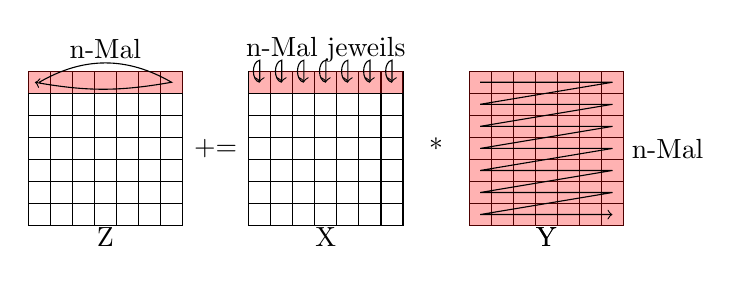
\begin{tikzpicture}[scale=0.28]
    % Matrix C
    \draw (0,0) rectangle (7,7);
    \foreach \i in {1,...,6} {
        \draw (\i,0) -- (\i,7);
        \draw (0,\i) -- (7,\i);
    }
    \foreach \i in {0,...,6} {
        \fill[red, opacity=0.3] (\i,6) rectangle (\i+1,7);
    }
    \node at (3.5,-0.5) {Z};

    % Loop symbol for Matrix C
    \draw[->] (0.5,6.5) to[bend left=30] (6.5,6.5) to[bend left=10] (0.3,6.5);
    \node at (3.5,8) {n-Mal};

    % += symbol
    \node at (8.5,3.5) {+=};

    % Matrix A
    \draw (10,0) rectangle (17,7);
    \foreach \i in {1,...,6} {
        \draw (10+\i,0) -- (10+\i,7);
        \draw (10,\i) -- (17,\i);
    }

    % Fill the first row with red color
    \foreach \i in {0,...,6} {
        \fill[red, opacity=0.3] (10+\i,6) rectangle (11+\i,7);
    }

    % Loop symbol for the first row of Matrix A
    \foreach \i in {0,...,6} {
        \draw[->] (10.5+\i,6.5) to[bend left=80] (10.5+\i,7.5) to[bend left=0] (10.5+\i,6.5);
    }
    \node at (13.5,8) {n-Mal jeweils};

    % Matrix name
    \node at (13.5,-0.5) {X};

    % * symbol
    \node at (18.5,3.5) {*};

    % Matrix B
    \draw (20,0) rectangle (27,7);
    \foreach \i in {1,...,6} {
        \draw (20+\i,0) -- (20+\i,7);
        \draw (20,\i) -- (27,\i);
    }
    \foreach \i in {0,...,6} {
        \foreach \j in {0,...,6} {
            \fill[red, opacity=0.3] (20+\i,6-\j) rectangle (21+\i,7-\j);
        }
    }
    % Matrix name
    \node at (23.5,-0.5) {Y};

    % Zigzag line with arrow
    \node at (23.5,-0.5) {Y};
    \draw[->] (20.5,6.5) -- (26.5,6.5) -- (20.5,5.5) -- (26.5,5.5) -- (20.5,4.5) -- (26.5,4.5) -- (20.5,3.5) -- (26.5,3.5) -- (20.5,2.5) -- (26.5,2.5) -- (20.5,1.5) -- (26.5,1.5) -- (20.5,0.5) -- (26.5,0.5);
    \node at (29,3.5) {n-Mal};

\end{tikzpicture}


In der zweiten Implementierung wird immer die Zeile übersprungen, 
wenn ein neues Element geladen wird. Dies führt dazu, 
dass die zweite Implementierung bei jedem neuen Element eine neue Cache Line laden muss. 
In Abbildung 12 ist das Verhalten der zweiten Implementierung dargestellt.\\
\textbf{Abbildung 12: Visualisierung der zweiten Implementierung}




\begin{adjustbox}{left}
    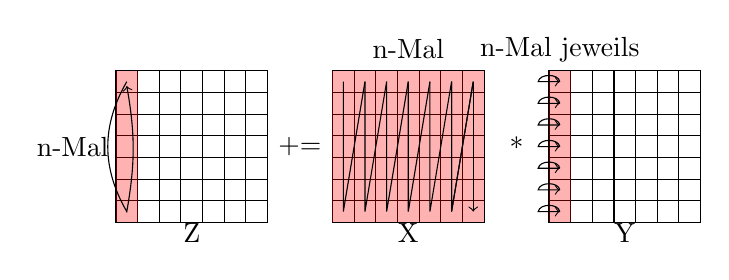
\begin{tikzpicture}[scale=0.275]
        % Matrix Z
        \draw (0,0) rectangle (7,7);
        \foreach \i in {1,...,6} {
            \draw (\i,0) -- (\i,7);
            \draw (0,\i) -- (7,\i);
        }
        \foreach \i in {0,...,6} {
            \fill[red, opacity=0.3] (0,\i) rectangle (1,\i+1);
        }
        \node at (3.5,-0.5) {Z};
    
        % Loop symbol for Matrix Z
        \draw[->] (0.5,6.5) to[bend right=30] (0.5,0.5) to[bend right=10] (0.5,6.3);
        \node at (-2,3.5) {n-Mal};
    
        % += symbol
        \node at (8.5,3.5) {+=};
    
        % Matrix X
        \draw (10,0) rectangle (17,7);
        \foreach \i in {1,...,6} {
            \draw (10+\i,0) -- (10+\i,7);
            \draw (10,\i) -- (17,\i);
        }
    
        % Fill all elements with red color
        \foreach \i in {0,...,6} {
            \foreach \j in {0,...,6} {
                \fill[red, opacity=0.3] (10+\i,\j) rectangle (11+\i,\j+1);
            }
        }
    
        % Zigzag line with arrow for Matrix X
        \foreach \i in {0,...,5} {
            \draw (10.5+\i,6.5) -- (10.5+\i,0.5) -- (11.5+\i,6.5);
        }
        \draw (15.5,6.5) -- (15.5,0.5) -- (16.5,6.5);
        \draw[->] (16.5,6.5) -- (16.5,0.5);
        \node at (13.5,8) {n-Mal};
    
        % Matrix name
        \node at (13.5,-0.5) {X};
    
        % * symbol
        \node at (18.5,3.5) {*};
    
        % Matrix Y
        \draw (20,0) rectangle (27,7);
        \foreach \i in {1,...,6} {
            \draw (20+\i,0) -- (20+\i,7);
            \draw (20,\i) -- (27,\i);
        }
        \foreach \i in {0,...,6} {
            \fill[red, opacity=0.3] (20,6-\i) rectangle (21,7-\i);
        }
        % Matrix name
        \node at (23.5,-0.5) {Y};
        \node at (20.5,8) {n-Mal jeweils};
    
        % Loop symbol for the first column of Matrix Y
        \foreach \i in {0,...,6} {
            \draw[->] (20.5,6.5-\i) to[bend right=80] (19.5,6.5-\i) to[bend right=0] (20.5,6.5-\i);
        }
        
        \end{tikzpicture}
        \end{adjustbox}


Bei ausreichend großen Matrizen kommt es zu ständigen Capacity Misses. 
Die Anzahl dieser kann einfach approximiert werden, 
indem man den einfachen Fall betrachtet, 
dass jeweils eine Zeile oder Spalte für Z, X und Y im Cache gehalten werden kann.
Es gibt $ \frac{\textnormal{n} \times \textnormal{n}}{\textnormal{L}} $ Cache Lines. 
Das erstmalige Laden jeder Cache Line für Z ist ein Cold Miss, 
aber die restlichen Zugriffe auf die gleiche Cache Line sind Capacity Misses. 
Das bedeutet, es gibt $\textnormal{n} * \textnormal{n} * \textnormal{n} - \frac{\textnormal{n} \times \textnormal{n}}{\textnormal{L}} $ 
Capacity Misses bei Z, wobei L die Anzahl der Elemente 
in einer Cache Line ist.
Bei X ist es ein ähnlicher Fall, da auch jedes Element nach einmaliger Nutzung in naher Zukunft verdrängt wird 
und später wieder benötigt wird. 
Es gibt also ebenfalls 
$\textnormal{n} * \textnormal{n} * \textnormal{n} - \frac{\textnormal{n} \times \textnormal{n}}{\textnormal{L}} $ 
Capacity Misses bei X.
Bei Y wird jedes Element n-Mal genutzt, bevor die Cache Line verdrängt wird. 
Daher kann man nur für jedes Element einen Capacity Miss zählen, 
mit Ausnahme des ersten Elemente jeder Cache Line. Anders ausgedrückt, 
es gibt $\textnormal{L} - 1 $ Capacity Misses pro Cache Line. 
Da es $ \frac{n \times \textnormal{n}}{\textnormal{L}} $ Cache Lines gibt, 
sind insgesamt $ \frac{\textnormal{n} \times \textnormal{n}}{\textnormal{L}} \times (\textnormal{L} - 1) $ Capacity Misses bei Y zu verzeichnen.
Insgesamt ergeben sich also 
$2 * \textnormal{n} * \textnormal{n} * \textnormal{n} - \frac{\textnormal{n} \times \textnormal{n}}{\textnormal{L}} + \frac{\textnormal{n} \times \textnormal{n}}{\textnormal{L}} \times (\textnormal{L} - 1) $ Capacity Misses.
Bei der ersten Implementierung hingegen gibt es keine Capacity Misses bei Z, 
da man stets eine Zeile für Z im Cache halten kann, ebenso wie bei X. 
Bei Y durchläuft man die Matrix zwar auch in Row-Major-Order, 
jedoch wird die erste Zeile nach der Bearbeitung der letzten verdrängt sein.
In der ersten Implementierung iteriert man n-Mal durch die Matrix Y. 
Der erste Durchlauf führt ausschließlich zu Cold Misses, 
während in den folgenden Durchläufen lediglich das erste Element jeder Cache Line einen Capacity Miss verursacht. 
Daher ergibt sich eine Gesamtzahl von $(\textnormal{n}-1) \times \frac{\textnormal{n} \times \textnormal{n}}{\textnormal{L}} $ Capacity Misses. 
Da die Anzahl der Capacity Misses bei der zweiten Implementierung deutlich höher ist, 
wird erwartet, dass die erste Implementierung, 
insbesondere bei großen Werten von \texttt{n}, eine bessere Performance aufweist.
In den Abbildungen 13 ist die Performance der beiden Implementierungen und die 4 restlichen 
Möglichkeiten der Matrix-Matrix Multiplikation dargestellt.\\\\ % Hier muss ein Quelle hin!!
\textbf{Abbildung 13: Performance der verschiedenen Implementierungen der Matrix-Matrix Multiplikation}
\\\\\\\\
Die zeitlichen Werte für die beiden vorgestellten Implementierungen, 
die auf dem i7-9700K Prozessor erzielt wurden, sind in Abbildung 14 dargestellt.
\textbf{Abbildung 14: Vergleich der beiden Implementierungen der Matrix-Matrix Multiplikation auf dem i7-9700K}
\\\\
In beiden Abbildungen ist zu erkennen das die Analyse der Zugriffsmuster und die Berechnung der Capacity Misses
einen guten Hinweis darauf geben können welcher Code effizienter arbeitet und das das Zugriffsmuster starken
Einfluss auf die Performance hat.



%%
%% The acknowledgments section is defined using the "acks" environment
%% (and NOT an unnumbered section). This ensures the proper
%% identification of the section in the article metadata, and the
%% consistent spelling of the heading.
\begin{acks}

\end{acks}

%%
%% The next two lines define the bibliography style to be used, and
%% the bibliography file.
\bibliographystyle{ACM-Reference-Format}
\bibliography{sample-base}


%%
%% If your work has an appendix, this is the place to put it.
\appendix



\end{document}
\endinput
%%
%% End of file `sample-acmtog.tex'.
